\chapter{LANs and VLANs}

\section{Historical background}

\subsection{Origins of wide area and local area networks}

Wide area networks emerged in the 1960s, when computing resources were concentrated in a limited number of mainframe installations. Terminals and remote systems required long distance connectivity to share the computational capabilities of these costly machines. Connecting multiple organizations to the same mainframe reduced operational expenses and justified the deployment of dedicated wide area links.

Local area networks developed later, in the late 1970s and early 1980s, alongside the diffusion of minicomputers and eventually personal computers. These systems were inexpensive enough to be deployed within small workgroups or departments, reducing the need to access remote mainframes for everyday tasks. Mainframes remained in use for computationally intensive applications such as scientific simulation, but LANs provided efficient shared access to local resources such as printers, file servers, and application servers.

\subsection{Early coexistence of heterogeneous technologies}

Initially, WAN and LAN technologies evolved independently. Different vendors engineered incompatible protocol suites intended for distinct environments and usage scenarios. Examples include DECnet and SNA for wide area environments, and Novell NetWare, Banyan VINES, and NetBEUI for local area communication.

As organizations attempted to interconnect LANs and WANs, the need for protocol unification increased. Over time, Internet Protocol became the dominant network layer solution and superseded competing architectures. The consolidation around IP facilitated seamless integration between local and wide area environments.

\section{LAN devices}

Local area networks rely on several classes of devices that operate at different layers of the protocol stack.

\subsection{Layer 1 devices}

\subsubsection*{Repeaters}
\addcontentsline{toc}{subsubsection}{Repeaters}

Repeaters operate at the physical layer. They receive a stream of bits, regenerate the signal, and retransmit it. Repeaters connect segments that share the same medium access control mechanism. In some cases, physical layer technologies may differ while the MAC layer remains identical.

Repeaters extend the maximum physical length of a network by compensating for signal attenuation. They do not create new collision domains; rather, all interconnected segments remain part of a single collision domain.

\begin{center}
\safeimg[width=3.54306in,height=1.25278in]{media/image16.png}
\end{center}

\subsubsection*{Hubs}
\addcontentsline{toc}{subsubsection}{Hubs}

Hubs are multiport repeaters. Their topology resembles a hub and spoke structure. Frames arriving on any port are broadcast to all other ports, preserving a single collision domain.

\begin{center}
	\safeimg[width=2.3625in,height=1.54028in]{media/image17.png}
\end{center}


The term \textit{hub-and-spoke topology}, commonly taught in basic networking courses, takes its name directly from these multiport repeaters, as multiple devices are connected to the distinct ports of a single central hub.  

Since a hub cannot break the collision domain, while one device is transmitting no other device can transmit in parallel without causing a collision. A hub can unify different physical domains, as long as they use the same medium access control algorithm. 
\subsection{Layer 2 devices}

\subsubsection*{Bridges and switches}
\addcontentsline{toc}{subsubsection}{Bridges and switches}

Bridges operate at the data link layer and interconnect LAN segments that may use different physical layer technologies or distinct MAC formats. For example, a bridge may connect an Ethernet network to a wireless LAN or link Ethernet and Fast Ethernet segments.

Bridges create separate collision domains while retaining a single broadcast domain. Modern bridges are implemented as switches and include hardware acceleration for forwarding decisions.

\begin{center}
	\safeimg[width=3.54306in,height=1.25278in]{media/image105.png}
\end{center}

It is crucial to remember that while bridges and switches successfully segment collision domains, they merge all connected segments into a single, unified \textbf{broadcast domain}, unlike routers

\begin{center}
	\safeimg[width=4.54306in,height=2.25278in]{media/image106.png}
\end{center}

\subsection{Layer 3 devices}

Routers operate at the network layer. They separate broadcast domains and forward packets based on network layer addresses. Although routers can be used in LANs, they are not specific to LAN environments and are not the focus of the present discussion.

\section{Collision and broadcast domains}

A collision domain is the region of a LAN in which a single medium access control algorithm operates. A collision domain corresponds to a contiguous physical segment, possibly extended through repeaters, in which all stations must coordinate access to the shared medium. In traditional Ethernet using CSMA/CD, simultaneous transmissions within a collision domain result in collisions detectable by all participating stations.

A \textbf{physical domain} is a part of a network built with a single type of physical medium, for example only coaxial cables or only fiber optic cables. A collision domain may include several physical domains. A collision occurs when multiple transmissions overlap: the signals of different frames are superimposed and the destinations cannot interpret the received bits. A medium access control algorithm either detects and manages collisions, as CSMA/CD does in Ethernet, or avoids them, as CSMA/CA does in Wi-Fi; whatever the approach, its goal is to provide correct communication. A collision domain is also called a \textit{network segment}.

A broadcast domain is the region in which link layer frames can be propagated. A broadcast domain may consist of multiple collision domains interconnected by bridges or switches. Frames can be buffered and retransmitted across collision domains, enabling the distribution of broadcast and multicast traffic.

When the extent of a LAN is considered, one typically refers to its broadcast domain, which is composed of multiple network segments, each one corresponding to a collision domain.

Routers separate broadcast domains by design; bridges do not.

\section{Repeaters}

Repeaters perform bit level regeneration and propagate signals through extended physical domains. They are useful when segments employ the same MAC procedure but require different physical signalling mechanisms or greater reach.

A repeater forms a single collision domain across all attached segments. For example, a coaxial cable segment may be connected to a fiber optic segment through a repeater, forming a single domain that shares collisions.




\begin{center}
	\safeimg[width=4.54306in,height=2.25278in]{media/image92.png}
\end{center}


As an example, consider hosts $H_1$, $H_2$ and $H_3$ on a coaxial segment and hosts $H_4$, $H_5$ and $H_6$ on a fiber optic segment, connected by a repeater. If $H_1$ sends a frame to $H_4$, the repeater repeats the bits on the other side, so that $H_4$, $H_5$ and $H_6$ receive them, but only $H_4$ keeps the frame, because it recognizes its own MAC address as destination. If $H_1$ sends a frame to $H_3$, the repeater still repeats it to $H_4$, $H_5$ and $H_6$: it sees only a sequence of bits, without understanding how they are organized into frames, so it cannot know that the destination is on the same side. Finally, if $H_1$ sends a frame to $H_3$ while $H_4$ sends a frame to $H_6$, the two transmissions collide on both sides, because the whole network is a single collision domain made of two physical domains. A repeater may also change the way the bits are represented from the analog point of view, for instance when it connects a copper cable to a fiber.



\section{Bridges}

\subsection{General characteristics}

Bridges were introduced in 1983 and initially implemented in software. Early bridges typically had two ports for economic reasons. They operate at the data link layer and may interconnect segments with different medium access mechanisms or frame formats.

Bridges form separate collision domains but maintain a unified broadcast domain. Broadcast and multicast frames propagate across the entire bridged network unless filtered explicitly.

Since a bridge works at the data link layer, it understands frames and can apply a store-and-forward mechanism: it receives a frame, stores it and forwards it only where needed. Consider the previous example with a bridge instead of the repeater. A frame from $H_1$ to $H_3$ is not repeated on the other side, because the bridge knows that $H_3$ is on the same side as $H_1$; therefore $H_4$ can send a frame to $H_6$ at the same time without any collision. Collisions can still occur, but only inside each collision domain, where the medium access control algorithm manages them: the bridge can send the frame on each side and afterwards detect any collision that may occur there. Many kinds of bridges exist, for instance only for Ethernet, only for wireless networks, or interconnecting Ethernet and Wi-Fi; the more different the interconnected collision domains are, the more complex the bridge is.

\subsection{Switched Ethernet}

Modern wired LANs rely on full duplex operation and switching, forming Switched Ethernet. Current speeds include gigabit Ethernet and higher. When discussing switches, the default assumption is an Ethernet switch.

In this course we focus on Ethernet bridges, which are commonly called switches: the terms bridge and switch are therefore used interchangeably.

Wireless LANs are based on completely different access mechanisms such as CSMA/CA. Although hubs still exist in specialized applications, such as wireless range extenders, switched Ethernet dominates contemporary wired networks.

\subsection{Transparent bridges}

Ethernet bridges are specified as transparent bridges in IEEE 802.1D. Transparency requires that bridges be entirely invisible to end systems. End nodes must use the same frame formats, MAC addresses, and operational procedures regardless of whether bridges are present. No changes are permitted in the encapsulation, source and destination addresses, or frame handling by the hosts.


Transparency concerns functionality, not performance. The presence of a bridge may affect performance, because of the store-and-forward operation and of the lookups in the forwarding table, which slightly delay the communication; this does not make the bridge non-transparent, since frames are created and received exactly as if the bridge did not exist, with the same source and destination MAC addresses and the same format. 

\begin{center}
	\safeimg[width=4.54306in,height=2.25278in]{media/image115.png}
\end{center}

For instance, a frame from $H_1$ to $H_2$ is identical whether the two hosts are connected through a hub or through an Ethernet switch. A router, in contrast, is not transparent: the MAC addresses of a frame change at every hop, whereas a frame may cross hundreds of switches without ever being modified; at most it is delayed by their processing.
\section{Components of a transparent bridge}

To function without manual configuration, a transparent bridge requires three components:

\begin{enumerate}
\item a local forwarding table, known as a filtering database;
\item an automatic learning mechanism, known as backward learning;
\item loop detection and avoidance, implemented through the spanning tree algorithm.
\end{enumerate}

These components enable the bridge to operate in a strictly \textbf{plug-and-play} manner, meaning absolutely zero manual configuration is required by the user or network administrator to begin forwarding frames.

\subsection{The filtering database}

The filtering database associates MAC addresses with bridge ports. Each entry consists of:

\begin{itemize}
\item a MAC address;
\item the corresponding outgoing port;
\item an ageing timer, after which the entry expires (typically 300 seconds).
\end{itemize}

Initially, filtering databases were perceived as mechanisms to filter unnecessary traffic from links. Modern implementations maintain the table dynamically for efficient forwarding.

\begin{center}
	\safeimg[width=4.54306in,height=2.25278in]{media/image116.png}
\end{center}

The name \emph{filtering} comes from the fact that a switch can decide not to forward a frame. For example, if a frame from $H_1$ to $H_2$ arrives on port 1 and the entry of $H_2$ also points to port 1, the switch filters the frame, because the destination has already received it; a frame from $H_1$ to $H_3$, reachable through port 2, is instead forwarded on port 2 only. The ageing timer of an entry is restored every time a new frame with that source address is received, so an entry remains in the database only as long as the device is active.

Switches include commands to inspect the filtering database. For example:

\begin{center}
	\safeimg[width=4.54306in,height=2.25278in]{media/image107.png}
\end{center}



\subsection{Forwarding process}

When a bridge receives a frame on port $X$, the following operations occur:
\begin{enumerate}
\item if the frame contains errors (such as CRC errors), it is discarded;
\item if the destination MAC address exists in the filtering database, let the associated port be $Y$:
\begin{itemize}
\item if $Y = X$, the frame is discarded because forwarding it on the receiving port is unnecessary;
\item if $Y \neq X$, the frame is forwarded only on port $Y$;
\end{itemize}
\item if the destination address is unknown, the switch performs \textbf{flooding}, meaning the frame is forwarded on all ports except $X$.
\end{enumerate}

The destination address of a frame may be unknown in several cases: a new device has been connected and has not sent any frame yet, the corresponding entry has expired, the switch has just been installed and its database is empty, or the frame is a broadcast or multicast frame, whose destination address does not represent a single host and is therefore never stored in the database. In all these cases the switch floods the frame.


\begin{center}
	\safeimg[width=4.54306in,height=2.25278in]{media/image108.png}
\end{center}


\textbf{Important Note:} The forwarding process relies \textit{exclusively} on the destination MAC address. The source MAC address is completely ignored during this phase and is never taken into account to make forwarding decisions. \textbf{This is a frequent source of mistakes and a typical topic of exam quizzes.}
   

\section{Backward learning}
The filtering database could in principle be populated manually, by writing every entry by hand. This is feasible but inefficient: in a LAN, devices are frequently moved from one position to another, so the entries would have to be updated continuously, whereas, for example, some routing tables are more static over time. An automatic control plane algorithm is therefore preferred, and it is called backward learning.

Backward learning updates the filtering database based on observed source addresses. When a frame with source address $S$ is received on port $P$, the bridge infers that $S$ is reachable via $P$. If the filtering database does not contain $S$, a new entry is added. If it does, the entry is updated and its ageing timer is reset.

\begin{center}
	\safeimg[width=4.54306in,height=2.25278in]{media/image109.png}
\end{center}

Backward learning ignores the destination address; it relies solely on the ingress port of each frame.

\begin{center}
	\safeimg[width=4.54306in,height=2.25278in]{media/image116.png}
\end{center}

As an example, consider a bridge with hosts $H_1$ and $H_2$ connected through port $P_1$ and hosts $H_3$ and $H_4$ through port $P_2$, with an empty filtering database. When $H_1$ sends a frame to $H_2$, the bridge writes only the entry ($H_1$, $P_1$): it does not write $H_2$, because it cannot know whether $H_2$ is on the left or on the right. When $H_3$ then sends a broadcast frame, the entry ($H_3$, $P_2$) is added. If later $H_3$ sends a frame to $H_4$, nothing changes, because the destination address is ignored.

When a frame is received from a source that is already in the database, the ageing timer is restored to its initial value (for instance 300 seconds), even if it had already reached, say, 120, because the switch understands that the host is still active and must remain reachable. If the frame arrives on a different port from the one stored, the bridge concludes that the host has moved and updates the port in the entry. Entries whose ageing timer expires are removed by a background process, so that no \emph{zombie} entries remain for hosts that are no longer in the network.

\subsection{Operation in multi-bridge networks}

Backward learning works across multiple bridges. When a host transmits a frame, each bridge along the path records the host's location. Remote bridges learn the position of end systems even when those end systems are not locally attached. This allows dynamic discovery of the entire bridged topology.

Each bridge stores only local information, that is, its own port numbers. 

\begin{center}
	\safeimg[width=4.54306in,height=2.25278in]{media/image118.png}
\end{center}

For instance, when $H_1$ sends a broadcast frame across three bridges, each bridge records $H_1$ together with the port from which the frame arrived at that bridge, so each bridge learns in which direction $H_1$ is. Even if some copies of the frame are useless for the communication that generated them, this propagation is useful for learning, because it lets the bridges know immediately the position of the host.

\subsection{Transient learning phase}

When a bridge starts up or when previously unknown nodes appear, the filtering database may be empty. In this transient state, the bridge floods all frames except on the receiving port. As more frames are observed, the database fills and selective forwarding begins.

During this phase the bridge behaves as a repeater (or, with several ports, as a hub): every frame reaches every part of the network, as if all frames were broadcast frames.


In this transient state, the bridge applies a technique known as \textit{MAC flooding}, replicating all frames on every port except the receiving one. This situation must be temporarily accepted until the database fills and selective forwarding begins, but it is precisely this fallback mechanism that gets exploited maliciously during a MAC flooding attack.

\subsection{Attacks on the filtering database}

A MAC flooding attack generates frames with random source MAC addresses in an attempt to exhaust the switch's filtering database. When the database reaches its capacity, the switch may no longer have space to learn new source MAC addresses. Consequently, destination addresses that are not present in the database are treated as unknown, and the switch resorts to flooding frames on all ports except the receiving port.

This behavior makes the switch resemble a hub, increasing congestion and potentially exposing traffic to interception. The attack is a denial-of-service (DoS) attack because it degrades the normal forwarding behavior of the switch and may impair network availability.

Some switch implementations allow administrators to limit the number of MAC addresses learned per port. For example, a maximum of 200 addresses may be configured for a port. This can limit the amount of filtering database capacity consumed by devices connected through that port and help protect the resources available for legitimate hosts elsewhere in the network.

This defense is effective because an attacker is physically connected to a single port and cannot easily move to other ports: after the attacker has sent 200 frames with random source MAC addresses, the counter of that port is exhausted and no more entries are added for frames coming from it, so the space available for the hosts connected to the other ports is preserved.

\section{Bridges in meshed topologies}

Backward learning alone does not prevent loops. In networks containing redundant links or cycles of bridges, frames may circulate indefinitely. Two critical problems arise:

\begin{itemize}
\item broadcast storms, where broadcast or multicast frames are forwarded repeatedly around loops;
\item unstable filtering databases, where entries oscillate between ports and never reach a stable configuration.
\end{itemize}

Because Ethernet frames lack a time to live field, bridges cannot rely on automatic expiration to suppress loops. Disabling physical links is the only intrinsic solution unless loop detection mechanisms are deployed.

\subsection{Broadcast storms}

Broadcast storms consist of uncontrolled flooding of broadcast or multicast traffic, but they can also be triggered by frames addressed to non-existing stations. For instance, an attacker could continuously send frames with random \textit{destination} MAC addresses; since these addresses will never be learned by the filtering databases, the switches will permanently flood them. These storms can saturate available bandwidth, cause severe network loops, and render the LAN unusable. Network operators have limited options during a broadcast storm because no field within the Ethernet frame itself (such as a Time-To-Live) can prevent indefinite circulation.


\begin{figure}[htbp]
	\centering
	% Immagine di sinistra: Broadcast frame
	\begin{subfigure}[b]{0.48\textwidth}
		\centering
		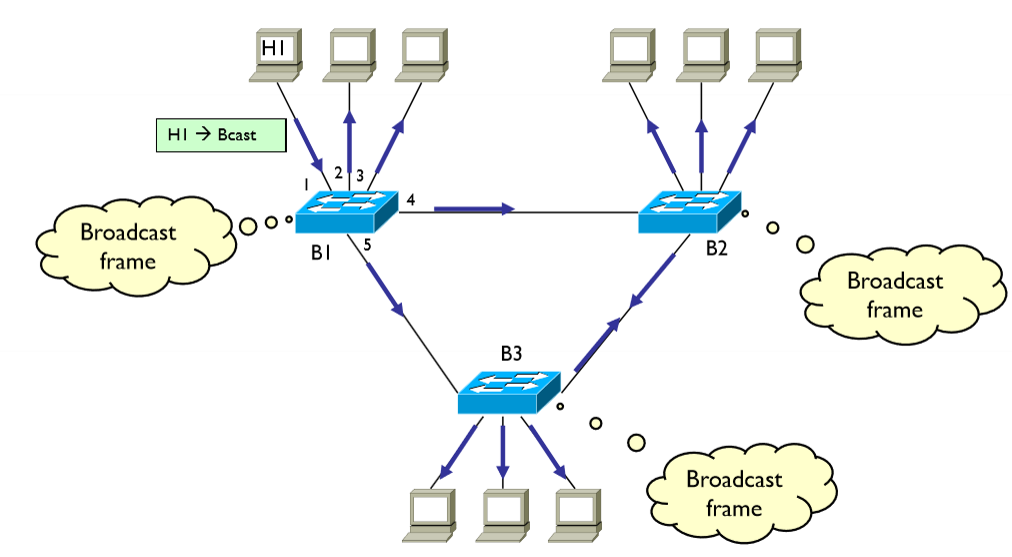
\includegraphics[height=3cm, keepaspectratio]{media/image110.png} 
		\caption{Time 1: Broadcast frame}
		\label{fig:broadcast_stage}
	\end{subfigure}
	\hfill
	% Immagine di destra: Loop
	\begin{subfigure}[b]{0.48\textwidth}
		\centering
		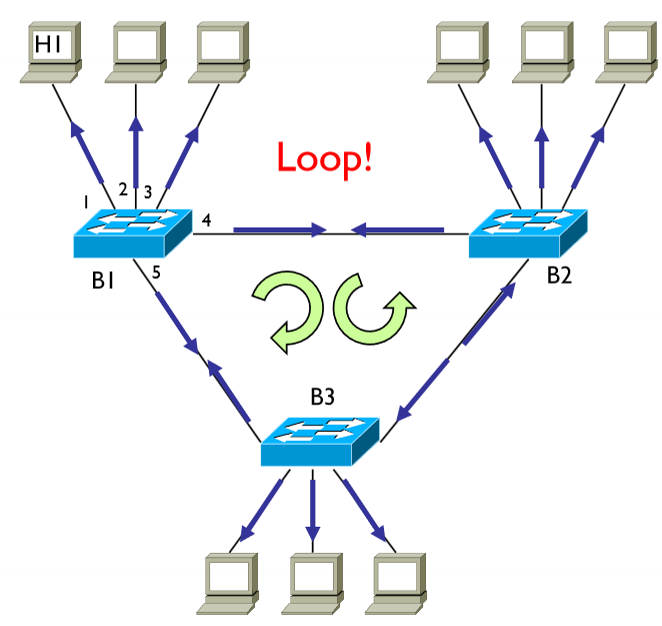
\includegraphics[height=3cm, keepaspectratio]{media/image111.png} 
		\caption{Time 2: Loop!}
		\label{fig:loop_stage}
	\end{subfigure}
	\caption{Comparison between the initial broadcast forwarding and the critical network evolution over time.}
	\label{fig:network_comparison}
\end{figure}

Multicast frames, which are less common in IPv4, are much more common in IPv6, so they contribute significantly to storms. Consider three bridges $B_1$, $B_2$ and $B_3$ interconnected in a triangle, with $H_1$ connected to $B_1$. When $H_1$ sends a broadcast frame, $B_1$ floods it on all ports except the receiving one, so a copy reaches $B_2$ and a copy reaches $B_3$. Each of them replicates it on its other ports and towards the other bridge; when $B_2$ and $B_3$ receive the copies coming from each other, they cannot recognize them as copies of a frame already received, since the Ethernet frame carries nothing that identifies it, and they flood them again towards $B_1$, which replicates them once more. The loop never stops unless one of the links is physically disabled.

A frame sent to a non-existing station loops for the same reason, but with a different cause: since that station never sends frames, its MAC address is never learned, and every switch keeps flooding the frame. This differs from the transient of a new switch, where entries are eventually learned as soon as the hosts send frames; typically, this situation occurs under an attack, such as the one with random destination MAC addresses described above.




This happens because the Ethernet header lacks a Time-To-Live (TTL) field. The inability to naturally discard looping frames at Layer 2 was historically one of the primary motivations for the creation of the IP protocol, which introduced the TTL (or Hop Limit) mechanism specifically to solve this issue at Layer 3.

Because of this structural limitation, a Layer 2 broadcast storm is exceptionally dangerous: it will rapidly consume all available bandwidth and switch CPU resources, inevitably bringing the entire LAN to a halt until the physical loop is broken or algorithmically blocked by STP
\subsection{Learning inconsistencies}

In a looped topology, backward learning may cause MAC entries to change ports repeatedly. When frames traverse the loop, each bridge may update its table incorrectly, causing persistent instability.

For instance, in the triangle of bridges, $B_1$ initially learns $H_1$ on the port towards $H_1$. Suppose the copy of the broadcast frame sent by $B_3$ comes back to $B_1$ before the one sent by $B_2$ (for example because $B_3$ is faster): $B_1$ receives a frame whose source is $H_1$ on the port towards $B_3$ and updates the entry, as if $H_1$ had moved, which is not true. A frame later sent by another host to $H_1$ would then be forwarded towards $B_3$, which is wrong. Shortly after, the copy coming from $B_2$ changes the entry again, and the entry keeps alternating between the two ports for as long as new copies arrive. The same happens in $B_2$ and $B_3$: besides saturating the bandwidth, the storm makes every bridge lose a correct view of the network. Since the two problems are connected, solving the loop solves both.

\section{Introduction to spanning tree}

To prevent loops, bridges implement the spanning tree algorithm. The algorithm identifies a subset of the physical topology that forms a loop free tree. Links not belonging to the spanning tree are disabled for data traffic. Broadcast and multicast frames propagate through the active tree, ensuring freedom from loops.

Routers, in contrast, separate broadcast domains and do not forward link layer broadcasts. They rewrite MAC addresses on forwarded frames and operate at the network layer. Different IP networks must be assigned to a router's interfaces to ensure correct forwarding semantics.


This logical disabling of links explains why STP is strictly suited for LANs and not WANs: in a WAN, automatically disabling an expensive intercontinental fiber-optic link to prevent loops would be an unacceptable waste of financial resources. In campus LANs, however, loops are often intentionally introduced by administrators to provide physical redundancy; if an active link fails, STP automatically detects the failure and restores the usage of a previously disabled link without requiring human intervention.

\begin{center}
	\safeimg[width=4.54306in,height=2.25278in]{media/image112.png}
\end{center}


The Spanning Tree Protocol (STP) is a protocol in its own right, through which the bridges interact with each other and decide, automatically, which link to disable logically; the choice is the result of an election among the bridges, based on the topology they discover. In the triangle example, the link between $B_2$ and $B_3$ could be disabled: broadcast frames, multicast frames and frames sent to non-existing stations are still flooded, but only along the remaining links, so they can no longer loop. Not all switches support STP, and the protocol exists in several variants (for example the Rapid Spanning Tree Protocol). It is a rather complex protocol, and its details are outside the scope of this course.

\section{Layer 2 versus layer 3 in campus networks}

\subsection{Considerations on protocol layer choice}

Until this point, the discussion has focused primarily on layer 2 mechanisms. A fundamental design question in campus networks concerns whether communication should remain at layer 2 or transition to layer 3.

Layer 2 operation provides transparency: end systems can communicate independently of their physical location within the LAN, and the network accommodates any protocol encapsulated in Ethernet frames. Layer 3 operation ties addressing to topology. Hosts receive IP addresses that depend on their position in the network, and many policies such as access lists and firewall rules are bound to the assigned IP prefixes.

When a device is moved from one network to another, at layer 3 its IP address changes, because it depends on its position, and routing tables may have to be updated; at layer 2 the MAC address is preserved, and backward learning simply updates the port in the filtering databases. Moreover, every function whose behavior depends on IP addresses must be updated whenever addresses change. For instance, a packet filtering firewall decides whether a packet is dropped by looking at the IP five-tuple, whose main elements are the source and destination IP addresses, so its access control list must be modified when a host receives a new address; the same holds for other access control functions, intrusion detection systems and, in general, any network security function based on IP addresses.


Furthermore, an L2 infrastructure natively works with any network protocol, allowing organizations or research laboratories to easily deploy and test experimental protocols (as was done during the early development of IPv6) without requiring hardware or routing software upgrades.

\section{Single versus multiple LANs in a campus}

\subsection{Motivation for multiple LANs}

It is generally preferable to maintain layer 2 operation as long as feasible. However, a single unified LAN may become impractical due to scalability constraints inherent in layer 2 networks.

Several issues motivate the subdivision of a campus into multiple LANs:

\begin{itemize}
\item \emph{performance}: broadcast traffic is not filtered by switches, so a single large broadcast domain can experience excessive broadcast or flooded traffic, especially during spanning tree reconfigurations;
\item \emph{privacy and security}: isolation between groups of users is desirable to contain potential information leakage or mitigate attacks such as MAC flooding;
\item \emph{management}: smaller networks are easier to administer, and per group or per department policies can be applied uniformly.
\end{itemize}

These motivations follow the divide-and-conquer paradigm (\emph{divide et impera}): it is better to have several smaller LANs, each independently managed, than a single large one. For instance, if a MAC flooding attack, or a flow of frames with random destination MAC addresses, targets a single large LAN, all its switches are affected; if the network is divided into several LANs interconnected by routers, the attack only affects the switches of the targeted LAN.

\subsection{Physical separation versus virtual segmentation}

One approach to creating multiple LANs is to deploy physically separate networks. If \(N\) LANs must span \(M\) rack rooms, the number of required switches becomes \(N \times M\), and the number of interconnecting links becomes \(N \times (M - 1)\). This strategy wastes resources and complicates maintenance.

To solve the single broadcast domain problem, the classic solution consists of dividing the network into separate subnets and assigning dedicated hardware (separate switches) to each department.

If a commercial switch has 24 or 48 physical ports but a department only has 4 or 5 hosts, most of the switch's physical ports remain unused. Multiplying this scenario for each department, infrastructure costs and hardware waste become unsustainable.

Virtual LANs provide a more efficient alternative.

\section{Virtual LANs}
\subsection{Concept and motivation}

A Virtual LAN (VLAN) allows multiple logical LANs to coexist on a single physical network infrastructure. The same switches and cabling can support multiple departments or groups while dividing the network into separate, logically isolated broadcast domains.

\begin{center}
	\safeimg[width=4.54306in,height=2.25278in]{media/image93.png}
\end{center}

VLAN membership is determined by the configuration of switch ports rather than by physical wiring. From a logical perspective, each VLAN behaves as an independent and isolated transparent bridge, maintaining its own separate filtering database and broadcast domain, while sharing the underlying physical hardware with other VLANs

Main advantages:

\begin{itemize}
\item \textbf{Infrastructural efficiency:} VLANs maximize the utilization of physical switch ports. For example, a single 48-port switch can serve multiple departments simultaneously, avoiding the need for dedicated physical switches for each group.

\item \textbf{Reduced backbone complexity:} Multiple VLANs can share the same physical backbone infrastructure, eliminating the need for multiple parallel backbone links dedicated to separate LANs.

\item \textbf{Broadcast domain isolation:} Broadcast frames generated by a host remain confined to its own VLAN and are not forwarded across VLAN boundaries. This reduces unnecessary broadcast traffic between departments.

\item \textbf{Layer 2 security and isolation:} VLANs limit the scope of certain Data Link layer attacks, such as MAC flooding and ARP spoofing (ARP poisoning). These attacks are generally confined to the affected VLAN and do not automatically propagate to other VLANs. However, VLANs alone do not guarantee complete security and must be combined with appropriate network security mechanisms.

\item \textbf{Organizational flexibility:} Users can be assigned to different logical networks independently of their physical location. For example, when a user moves to another office, the switch port can be reconfigured to assign the user to the same VLAN, without requiring changes to the physical cabling infrastructure.

\end{itemize}

Overall, VLANs provide logical network segmentation over shared physical infrastructure, improving resource utilization, reducing broadcast traffic, simplifying network design, and enabling flexible network administration.

\subsection{VLAN aware switch architecture}

A VLAN-aware switch maintains conceptually separate filtering databases, one for each VLAN. Each database associates MAC addresses with the local switch ports through which the corresponding devices can be reached within that VLAN. Backward learning is also performed independently for each VLAN, so information learned from a frame belonging to one VLAN does not modify the filtering database of another VLAN.

This logical separation is essential because VLANs represent distinct broadcast domains even when they share the same physical switches and cabling infrastructure. Consequently, a switch must identify the VLAN to which an incoming frame belongs before applying backward learning and forwarding decisions.
\begin{center}
	\safeimg[width=4.54306in,height=2.25278in]{media/image94.png}
\end{center}

In practical implementations, the filtering database is often a unified hardware table, frequently implemented using ternary content addressable memory. Entries include additional fields that identify the VLAN context.

\subsubsection{Filtering Databases and Forwarding in VLANs} 

Furthermore, the Spanning Tree Protocol (STP) computes a loop-free subset of the network topology. The following example illustrates how a VLAN-aware switch forwards frames between hosts belonging to the same VLAN while preventing direct Layer 2 communication between different VLANs.

\begin{center}
	\safeimg[width=5.54306in,height=3.25278in]{media/image113.png}
\end{center}

Consider the image before ,the network composed of two switches and six hosts, divided into three VLANs represented by green, yellow, and pink. The hosts are paired as follows: H1 and H4 belong to the green VLAN, H2 and H5 belong to the yellow VLAN, and H3 and H6 belong to the pink VLAN.

Each switch maintains a separate filtering database for each VLAN. When switch 1 receives a frame from H1 destined for H4, it identifies the frame as belonging to the green VLAN and consults only the green filtering database. Since H4 is associated with the appropriate output port in that database, switch 1 forwards the frame through that port. The next switch performs the same operation using its own green filtering database and forwards the frame toward H4. The destination is therefore reached without consulting the databases associated with the other VLANs.

Now suppose that H1 sends a frame destined for H6. Switch 1 again identifies the VLAN associated with the incoming frame and consults only the corresponding filtering database. The entry for H6 is not available in that VLAN's database because H6 belongs to the pink VLAN. The switch must not use the pink database to forward a frame that belongs to another VLAN. Consequently, the frame cannot reach H6 through Layer 2 forwarding.

This behavior is intentional: a VLAN defines a separate broadcast domain, and Layer 2 frames cannot cross VLAN boundaries directly. Communication between different VLANs requires an intermediate Layer 3 device, such as a router.

Without inter-VLAN routing, the only communicating host pairs in this example are H1–H4, H2–H5, and H3–H6. Other pairs belong to different VLANs and cannot communicate directly at Layer 2.

Although these filtering databases are logically independent, they do not necessarily require physically separate memory devices. In practical switches, entries may be stored in a common hardware table, with additional information identifying the VLAN associated with each entry. The switch uses this VLAN context to access the appropriate logical database and preserve traffic isolation.

\section{Interconnecting VLANs}

\subsection{Layer 2 separation}

Layer 2 frames do not cross VLAN boundaries. A host cannot send a link layer frame directly to a station in another VLAN. As VLANs define separate broadcast domains, flooded and broadcast traffic remains confined. Therefore, VLANs require a layer 3 device for interconnection.

Broadcast domains cannot be separated by repeaters, nor by switches, but only by routers. Since VLANs are separate broadcast domains, layer 2 frames cannot cross from one VLAN to another without an intermediate network layer device.

This behavior enforces the fundamental rule of VLANs: a Data Link frame can never pass directly from one VLAN to another within an L2 switching infrastructure. If a host attempts to send an L2 frame directly to a device in a different VLAN, the switch consults only the filtering database of the ingress VLAN, fails to find the destination MAC address in that specific context, and either discards the frame or floods it exclusively within the source VLAN.

\subsection{Inter-VLAN routing}
Inter VLAN communication requires a router or a device with equivalent layer 3 forwarding capability. In a traditional approach, every VLAN requires a dedicated physical switch port connected to a separate physical router interface, leading to severe port wastage and poor scalability.


\begin{center}
	\safeimg[width=4.54306in,height=2.25278in]{media/image95.png}
\end{center}

The main limitation of the traditional approach is the number of physical switch ports reserved for the router. For example, watching the image above, consider a 16-port switch that must support 10 VLANs. If one dedicated port is required for each VLAN, 10 of the 16 ports must be reserved for connections to the router, leaving only 6 ports available for other connections. This represents a significant waste of resources. By contrast, if the switch manages only two VLANs, dedicating two ports to the router may be an acceptable solution.

An alternative is the one-arm router, also known as router-on-a-stick. In this configuration, a single physical link connects the switch to one router interface, reducing the number of reserved switch ports. However, because frames belonging to different VLANs arrive through the same physical interface, the router cannot identify the VLAN solely from the incoming port. It must use additional information carried by the frames, typically VLAN tags, to distinguish the different VLANs.

The router can configure multiple logical subinterfaces on the same physical interface, assigning a different IP address to each subinterface. Each subinterface acts as the Layer 3 gateway for its corresponding VLAN. This solution reduces physical port consumption but increases configuration and management complexity because multiple logical interfaces and IP addresses must be maintained on a single physical connection.

When routing traffic between VLANs, the router examines the destination IP address, decapsulates the incoming layer 2 frame, and completely constructs a new frame. This process includes generating new source and destination MAC addresses (where the source becomes the router's interface MAC and the destination belongs to the final target host) and applying the appropriate 802.1Q VLAN tag before re-injecting the frame back onto the shared trunk link.

\subsubsection{VLANs and IP addressing}
Because ARP broadcasts and other discovery protocols cannot cross VLAN boundaries, each VLAN must correspond to a distinct IP subnet. Hosts belonging to different VLANs require addresses from different IP prefixes. Consequently, assigning overlapping IP subnets to different VLANs constitutes a severe design error, as Layer 2 forwarding rules will block direct communication even if hosts appear to share the same logical subnet prefix. 

\begin{center}
	\safeimg[width=3.84306in,height=1.65278in]{media/image114.png}
\end{center}

Inter VLAN routing is then performed according to standard IP forwarding rules, relying on the router's subinterfaces as the default gateways for each respective network segment.

\section{Association of frames to VLANs}

\subsection{VLANs on a single switch}
When VLANs exist only within a single switch, the simplest method to associate incoming frames with VLANs is port-based assignment (also known as static VLANs). Each port is statically configured to belong to a specific VLAN, defining its Port VLAN ID (PVID). Incoming untagged frames are assigned by the switch to the VLAN configured on that port. This method requires no changes to end hosts, which remain completely transparent to the underlying logical segmentation.

\begin{center}
	\safeimg[width=4.54306in,height=2.25278in]{media/image96.png}
\end{center}


For example, suppose H1 and H3 are connected to the same VLAN-aware switch but their access ports are assigned to different VLANs. When H1 sends a frame addressed to H3, the switch associates the incoming frame with the VLAN configured on H1's port. It then consults only the filtering database of that VLAN. Even if H3 is connected to the same physical switch, the frame cannot be forwarded directly to H3 if H3 belongs to another VLAN. This illustrates that VLAN membership is determined by the switch configuration, rather than simply by physical connectivity.
\subsection{VLANs across multiple switches}

When VLANs span multiple switches, frames must be identifiable across inter switch links. A single physical link may carry traffic of multiple VLANs. Similarly, servers, routers, or other devices may belong to more than one VLAN and must be able to transmit VLAN tagged frames.

An inter-switch link cannot be treated as a regular access port assigned to a single VLAN when it must carry traffic belonging to multiple VLANs. If the link were assigned to only one VLAN, frames belonging to other VLANs would not be correctly associated with their respective broadcast domains. Assigning an additional VLAN to the same untagged link would not solve the problem, because the receiving switch identifies untagged frames according to the VLAN configured on the ingress port. Therefore, the link between switches must use VLAN tagging to preserve the identity of each frame's VLAN. The same requirement applies to servers and routers that need to communicate with multiple VLANs through a single physical interface.
\begin{center}
	\safeimg[width=4.54306in,height=2.75278in]{media/image97.jpg}
\end{center}

 To support these scenarios, a tagging mechanism is required. On the other hand, if inter-switch links are misconfigured—such as connecting two switches using Access ports set to different VLANs—no tags are used. This causes a dangerous security flaw called VLAN leaking, where computers from different VLANs accidentally communicate at Layer 2.

\subsection{IEEE 802.1Q tagging}

IEEE 802.1Q specifies an extension of the Ethernet frame format that inserts a 4 byte tag between the source MAC address and the EtherType or length field. 

\begin{center}
	\safeimg[width=4.54306in,height=2.75278in]{media/image98.png}
\end{center}


The tag contains:

\begin{itemize}
	\item \textbf{the Tag Protocol Identifier (TPID)}, set to the hexadecimal value 0x8100 to indicate an 802.1Q framed packet;
	\item \textbf{the Priority Code Point (PCP)} or user priority field (3 bits) for Layer 2 Quality of Service (CoS);
	\item \textbf{the Drop Eligible Indicator (DEI)} or CFI (1 bit) used for congestion management;
	\item \textbf{a 12-bit VLAN identifier (VID)} in the range 1 to 4094 (with 0 and 4095 reserved).
\end{itemize}

The EtherType value 0x8100 indicates that a VLAN tag follows. Tagged frames are therefore 4 bytes longer than standard untagged frames.

\begin{center}
	\safeimg[width=4.54306in,height=2.75278in]{media/image99.png}
\end{center}

Tagging is used only on links that transport multiple VLANs, such as inter-switch connections (trunk ports) or connections to servers, hypervisors, and routers that require membership in several VLANs. End-user devices (PCs) remain untagged at the edge, relying on the switch to add or strip tags transparently.

VLAN tagging is generally used in the network backbone, particularly on trunk links connecting switches, while ordinary end hosts usually exchange untagged Ethernet frames. This design choice preserves the transparency of the switching infrastructure: end systems can communicate without needing to know how VLANs are implemented internally.

The switches add, interpret, and remove VLAN tags when necessary, so that the endpoints can operate without managing VLAN identification themselves. If an endpoint generates tagged frames, it must be aware of the VLAN tagging mechanism and participate in the assignment process. This breaks the transparency normally provided by the switches.

Therefore, the design involves a trade-off. Keeping frames untagged at the network edge simplifies endpoint configuration and preserves transparency, whereas tagging is necessary on links that must carry traffic belonging to multiple VLANs. Some devices, particularly servers and one-arm routers, must generate and process tagged frames because they participate in several VLANs through a single physical connection.
\section{Port types}

\subsection{Access ports}

Access ports send and receive untagged frames, and they represent the default configuration mode for VLAN-aware switches. They are typically used at the edges of the local area network to connect end devices (such as PCs or printers) in order to preserve network transparency as much as possible. Incoming traffic is associated with the VLAN configured on the port, and end systems do not need to modify their frame format.

An access port typically connects a single endpoint or a subnetwork of several endpoints belonging to the same VLAN: whatever arrives through the port is tagged with the VLAN configured on it, regardless of which devices (for instance other VLAN-unaware switches) are behind it. If two access ports, even on different switches connected by a trunk link, are configured with the same VLAN, the two subnetworks belong to the same VLAN and therefore to the same IP network, since each VLAN is a broadcast domain, inside which all the devices must be able to reach each other directly, without passing through a router. As a consequence, if an exercise asks for the IP address range of the devices of such subnetworks, separate ranges cannot be used: the total number of devices must be counted, and a single range sized for the global number of devices must be chosen.


The VLAN assignment configured on access ports is local to each switch and does not propagate to other switches. However, using access ports on links that must carry multiple VLANs (such as inter-switch links) leads to misconfigurations where frames remain untagged across switches, causing unexpected communication between different VLANs.


\begin{center}
	\safeimg[width=3.54306in,height=1.75278in]{media/image100.png}
\end{center}
Consider two switches connected through access ports. The access port on switch 1 is assigned to VLAN 1, whereas the corresponding access port on switch 2 is assigned to VLAN 5. Suppose H1 is connected to switch 1 and H4 is connected to switch 2.

Although the two access ports have different VLAN assignments, these assignments are local to their respective switches. When H1 sends an untagged frame toward H4, switch 1 associates it with VLAN 1. The frame crosses the inter-switch link without a VLAN tag, because the link is configured as an access connection. Switch 2 receives the untagged frame and associates it with VLAN 5, according to its own local configuration.

Consequently, H1 may communicate with H4 even though the two hosts were intended to belong to different VLANs. This is an example of VLAN leaking, caused by an incorrect inter-switch configuration. To preserve VLAN separation across multiple switches, inter-switch links carrying several VLANs must be configured as trunk ports, so that each frame retains its VLAN identity.

\subsection{Trunk ports}

Trunk ports carry tagged frames and must be configured explicitly, as they are not the default mode. They are used for inter-switch connections (the network backbone) or for advanced devices that participate in multiple VLANs. A trunk port may transport traffic belonging to a configurable set of VLANs simultaneously by embedding the VLAN ID inside the frame headers.


Frames of different VLANs may pass through the same trunk port, so each frame must carry a tag: the layer 2 header must contain the VLAN ID, that is, the number representing the VLAN to which the frame belongs. The tag is added by a switch before sending the frame over the trunk link, and it is removed after receiving it from the trunk link. The port of a switch connected to a one-arm router is also a trunk port, because the router must manage frames belonging to different VLANs; it does so through cooperative assignment, that is, by tagging the frames it sends and removing the tag from the frames it receives. The same holds for a server that must interact at layer 2 with all the VLANs.
\begin{center}
	\safeimg[width=3.54306in,height=1.75278in]{media/image101.png}
\end{center}


\section{Methods for assigning hosts to VLANs}

Hosts may be assigned to VLANs in several ways:

\begin{itemize}
	\item port-based VLANs, where each port belongs to a single VLAN and handles untagged edge traffic;
	\item transparent assignment based on static associations between MAC addresses and VLANs;
	\item authentication-based assignment using IEEE 802.1X frameworks;
	\item cooperative assignment, where endpoints themselves generate tagged frames and participate in multiple VLANs.
\end{itemize}

The different VLAN assignment methods have different practical implications.

Port-based assignment is straightforward to configure and is widely used for ordinary end hosts. The switch associates each incoming untagged frame with the VLAN configured on the corresponding access port.

MAC-based assignment relies on static associations between device MAC addresses and VLANs. Although possible, it can be difficult to manage because administrators must maintain the associations as devices are added, replaced, or moved. For this reason, it is generally not the preferred solution.

Authentication-based assignment can use IEEE 802.1X, a mechanism also studied in Information System Security. Although it provides a way to associate devices with VLANs based on authentication, this approach is less commonly encountered in the scenarios considered in this lecture.

Cooperative assignment requires endpoints to generate and process VLAN-tagged frames themselves. This breaks the transparency normally provided by switches because the endpoints must be aware of VLAN identification.

However, cooperative assignment is mandatory for devices such as one-arm routers and servers that must participate in multiple VLANs through a single physical link. These devices need to identify the VLAN associated with each received frame and include the appropriate tag when generating frames for different VLANs. Other clients may also use cooperative assignment in special cases, but this is relatively uncommon; ordinary end hosts typically use access ports and untagged frames.

Devices such as servers or routers (like a one-arm router) that require membership in multiple VLANs must use trunk connections and perform cooperative assignment by generating VLAN-tagged frames.


\section{VLANs and spanning tree}

VLANs and the spanning tree algorithm are conceptually independent, but the spanning tree protocol must account for the network topology in which VLANs operate. Two approaches are possible.

In the first approach, a single spanning tree instance is computed for the entire LAN. When a link is disabled to prevent a Layer 2 loop, it is disabled for all VLANs. Consequently, the same loop-free topology is shared by every VLAN, even if some links could have been used by particular VLANs without creating a loop.

In the second approach, a separate spanning tree instance is computed for each VLAN. In this case, a link may be disabled for one VLAN while remaining active for another. Different VLANs can therefore use different loop-free subsets of the physical topology.

Both approaches are valid. The available options depend on the switch implementation and vendor. For example, the professor notes that Cisco switches use per-VLAN spanning tree in the implementations discussed in the lecture, whereas other switches may also support a single spanning tree instance for the entire LAN.

\begin{center}
	\safeimg[width=3.54306in,height=1.75278in]{media/image102.jpg}
\end{center}
\section{Limitations to VLAN isolation}

VLANs provide logical separation at the frame forwarding and broadcast domain level, but complete full network isolation is never guaranteed because the underlying physical infrastructure and inter-switch trunk links are shared. Consequently, broadcast frames and traffic from multiple VLANs must traverse these shared physical links. Therefore, if a broadcast storm occurs in one VLAN, the massive volume of traffic can saturate the physical bandwidth of the shared links, indirectly affecting and degrading the performance of other VLANs. Similarly, a MAC flooding attack can saturate these shared pathways even though it originates within a single VLAN.

Switches are classified into two main categories: VLAN-aware switches, which support VLAN tagging and frame processing, and VLAN-unaware switches (traditional unmanaged bridges). From an economic standpoint, VLAN-unaware switches are less expensive to produce and easier to manage, which is why they are predominantly used in domestic networks where users lack advanced networking expertise. Low-end consumer switches are frequently VLAN-unaware and may drop tagged frames as oversized.

On the contrary, enterprise environments heavily rely on professional products supporting VLAN tagging. However, it is quite common to find VLAN-unaware switches in corporate networks. Network managers typically deploy only professional equipment, but end users often face physical limitations—such as the necessity to attach multiple hosts to a single network socket—and tend to solve these issues independently by purchasing the cheapest unmanaged switches on the market.

Network administrators must anticipate and manage such scenarios to prevent possible network misbehaviour. However, VLAN-unaware switches can still be utilized effectively at the access layer (e.g., to add new ports), provided that all connected hosts belong to the exact same single VLAN.

In practice, the VLAN-unaware switch is connected to a single port of a VLAN-aware switch, which is configured as an access port marked with the single VLAN ID that represents the whole subnetwork below it. The subnetwork may contain several VLAN-unaware switches: what matters is that all the frames coming from it belong to the same VLAN, regardless of how many unaware switches they have crossed.
\begin{center}
	\safeimg[width=3.54306in,height=1.75278in]{media/image103.png}
\end{center}



VLAN isolation is therefore logical rather than physical. Although broadcast frames are confined to their respective VLANs at the endpoint level, traffic belonging to different VLANs may traverse the same trunk links. The bandwidth consumed by these shared links must account for the aggregate traffic of the VLANs using them.

Consequently, a broadcast storm or a MAC flooding attack originating in one VLAN may saturate shared physical links and indirectly degrade the performance of other VLANs. The other VLANs remain logically separated, but they can still be affected by congestion in the common infrastructure.
\section{Ethernet LAN design considerations}

Campus networks typically consist of an access layer (with switches deployed in rooms or on each floor connecting multiple devices via access ports), distribution layers, and core infrastructure. Trunk links interconnect switches transporting multiple VLANs simultaneously, as well as connecting data center servers. VLAN-unaware devices may appear at the edges but must be properly contained to avoid interfering with overall VLAN separation.

\begin{center}
	\safeimg[width=4.54306in,height=2.75278in]{media/image104.jpg}
\end{center}

Routers are required both for external Internet connectivity and for executing inter-VLAN routing. In typical campus designs, a single core router fulfills a dual role: serving as the default gateway for devices to reach the external network, and providing the necessary Layer 3 interconnectivity for devices belonging to different VLANs. Modern wired LANs are based on full-duplex switched Ethernet, where collision domains no longer exist and medium access control mechanisms such as CSMA/CD are obsolete. Redundant links increase robustness, and a spanning tree protocol maintains loop freedom across the topology.

\begin{notebox}
	\textbf{Exam note.} Exams typically contain an exercise on VLANs: a network topology is given together with the configuration of its ports (possibly an incorrect one) and the student must state which devices can communicate with each other, or how a given port must be configured. In most cases the answer follows directly from reading the figure and the configuration, applying the rules seen in this chapter.
\end{notebox}

\subsection{Example of an exam-style exercise}
%TODO ADD IMAGE - (Vedere quaderno 19/10/2026 - Example of exam exercise)
Consider two switches connected by an inter-switch link, with four hosts. Switch 1 has three access ports: a pink one connected to H1, a yellow one connected to H2, and a pink one connected to switch 2. Switch 2 has a green access port connected to switch 1, a green access port connected to H4 and a yellow access port connected to H3. The inter-switch ports are configured in access mode, not in trunk mode. This is not necessarily wrong, because in rare cases it may be used to consider a whole part of the network as a single VLAN, but in most scenarios it is the error to be detected.

Since there is no router, there is no distinction between layer 2 and layer 3 communication: it is enough to establish whether a communication is feasible. If there were a router, a question could instead ask whether a communication is feasible at layer 2 or at layer 3, and the answer would change depending on its presence. The six possible pairs are the following:
\begin{itemize}
	\item H1 and H2: not feasible, because their access ports on switch 1 belong to different VLANs (pink and yellow);
	\item H1 and H3: not feasible; the frame sent by H1 leaves switch 1 through the pink port and reaches switch 2 on a green port, but H3 is connected to a yellow port;
	\item H1 and H4: feasible; the frame reaches switch 2 on a green port and switch 2 sends it to H4, which is connected to a green port. Whether the configuration is correct depends on the intention of the administrator, but the communication is feasible;
	\item H2 and H3: not feasible, even though both access ports are yellow, because the VLAN ID of an access port has only local validity: using the same color, and therefore the same VLAN ID, on ports of different switches does not make them part of the same VLAN. Switch 1 drops the frame of H2, because all its other access ports are pink. This is the most common mistake in this kind of exercise;
	\item H2 and H4: not feasible;
	\item H3 and H4: not feasible, because they are connected to the same switch through access ports with different VLAN IDs.
\end{itemize}
Therefore, only the communication between H1 and H4 is allowed.

In general, VLAN exercises give a topology and ask to reason about the feasibility of communications, with access ports, trunk ports and possibly routers. Alternatively, given a scenario where two ports are not configured, they may ask how to configure them so that two hosts can communicate at layer 2 or at layer 3, or whether a one-arm router can be used in a specific scenario. They require reading the whole topology, but no calculations, unlike the exercises on IP address ranges.


